% =============================================================================
% Paper 1 — Figure: capability gate on the IPC fastpath
% =============================================================================
\documentclass[tikz,border=4pt]{standalone}
\usepackage{tikz}
\usetikzlibrary{positioning,arrows.meta,fit,backgrounds,calc}

\begin{document}

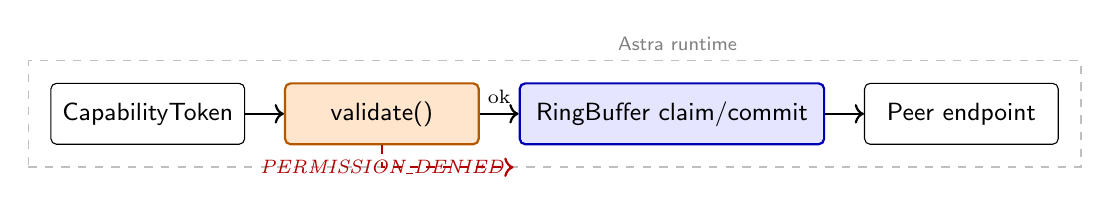
\begin{tikzpicture}[
    node distance=10pt and 14pt,
    box/.style    ={draw,rounded corners=2pt,minimum height=22pt,minimum width=70pt,
                    font=\small\sffamily,fill=white},
    gatebox/.style={box,fill=orange!20,draw=orange!70!black,thick},
    ringbox/.style={box,fill=blue!10,draw=blue!70!black,thick,minimum width=110pt},
    deny/.style   ={->,red!70!black,thick,dashed},
    pass/.style   ={->,black,thick}
]

\node[box]                                         (cap)    {CapabilityToken};
\node[gatebox, right=of cap]                       (gate)   {validate()};
\node[ringbox, right=of gate]                      (ring)   {RingBuffer claim/commit};
\node[box,     right=of ring]                      (peer)   {Peer endpoint};

\draw[pass] (cap)  -- (gate);
\draw[pass] (gate) -- node[above,font=\scriptsize]{ok} (ring);
\draw[pass] (ring) -- (peer);

\node[red!70!black,font=\scriptsize\itshape, below=2pt of gate] (deny)
    {PERMISSION\_DENIED};
\draw[deny] (gate.south) |- (deny.east);

\begin{scope}[on background layer]
    \node[fit=(cap)(peer), draw=gray!50, dashed, inner sep=8pt,
          label={[font=\scriptsize\sffamily,gray]above right:Astra runtime}] {};
\end{scope}

\end{tikzpicture}

\end{document}
